\section{Kết quả thực nghiệm}
Sau khi đã đi qua nền tảng lý thuyết của mạng NeuMiss, ta đi cài đặt và 
kiểm chứng các kết quả có đúng với lý thuyết hay không, dựa trên code của tác giả bài báo \footnote{Code của bài báo có tại \href{https://github.com/marineLM/NeuMiss}{https://github.com/marineLM/NeuMiss}}.

Toàn bộ code dùng để thực nghiệm trong bài báo cáo này được chạy trên Google Colab\footnote{\href{https://colab.research.google.com/}{https://colab.research.google.com/}},
có tại:
\href{https://github.com/ngntrgduc/seminar}{https://github.com/ngntrgduc/seminar}.


\subsection{Xấp xỉ ma trận bằng chuỗi Neumann}
Trước tiên, ta kiểm chứng độ hiệu quả cho việc xấp xỉ nghịch đảo ma trận nửa xác định dương, với bán kính phổ bé hơn $1$ bằng chuỗi Neumann.

\begin{figure}[h]
    \centering
    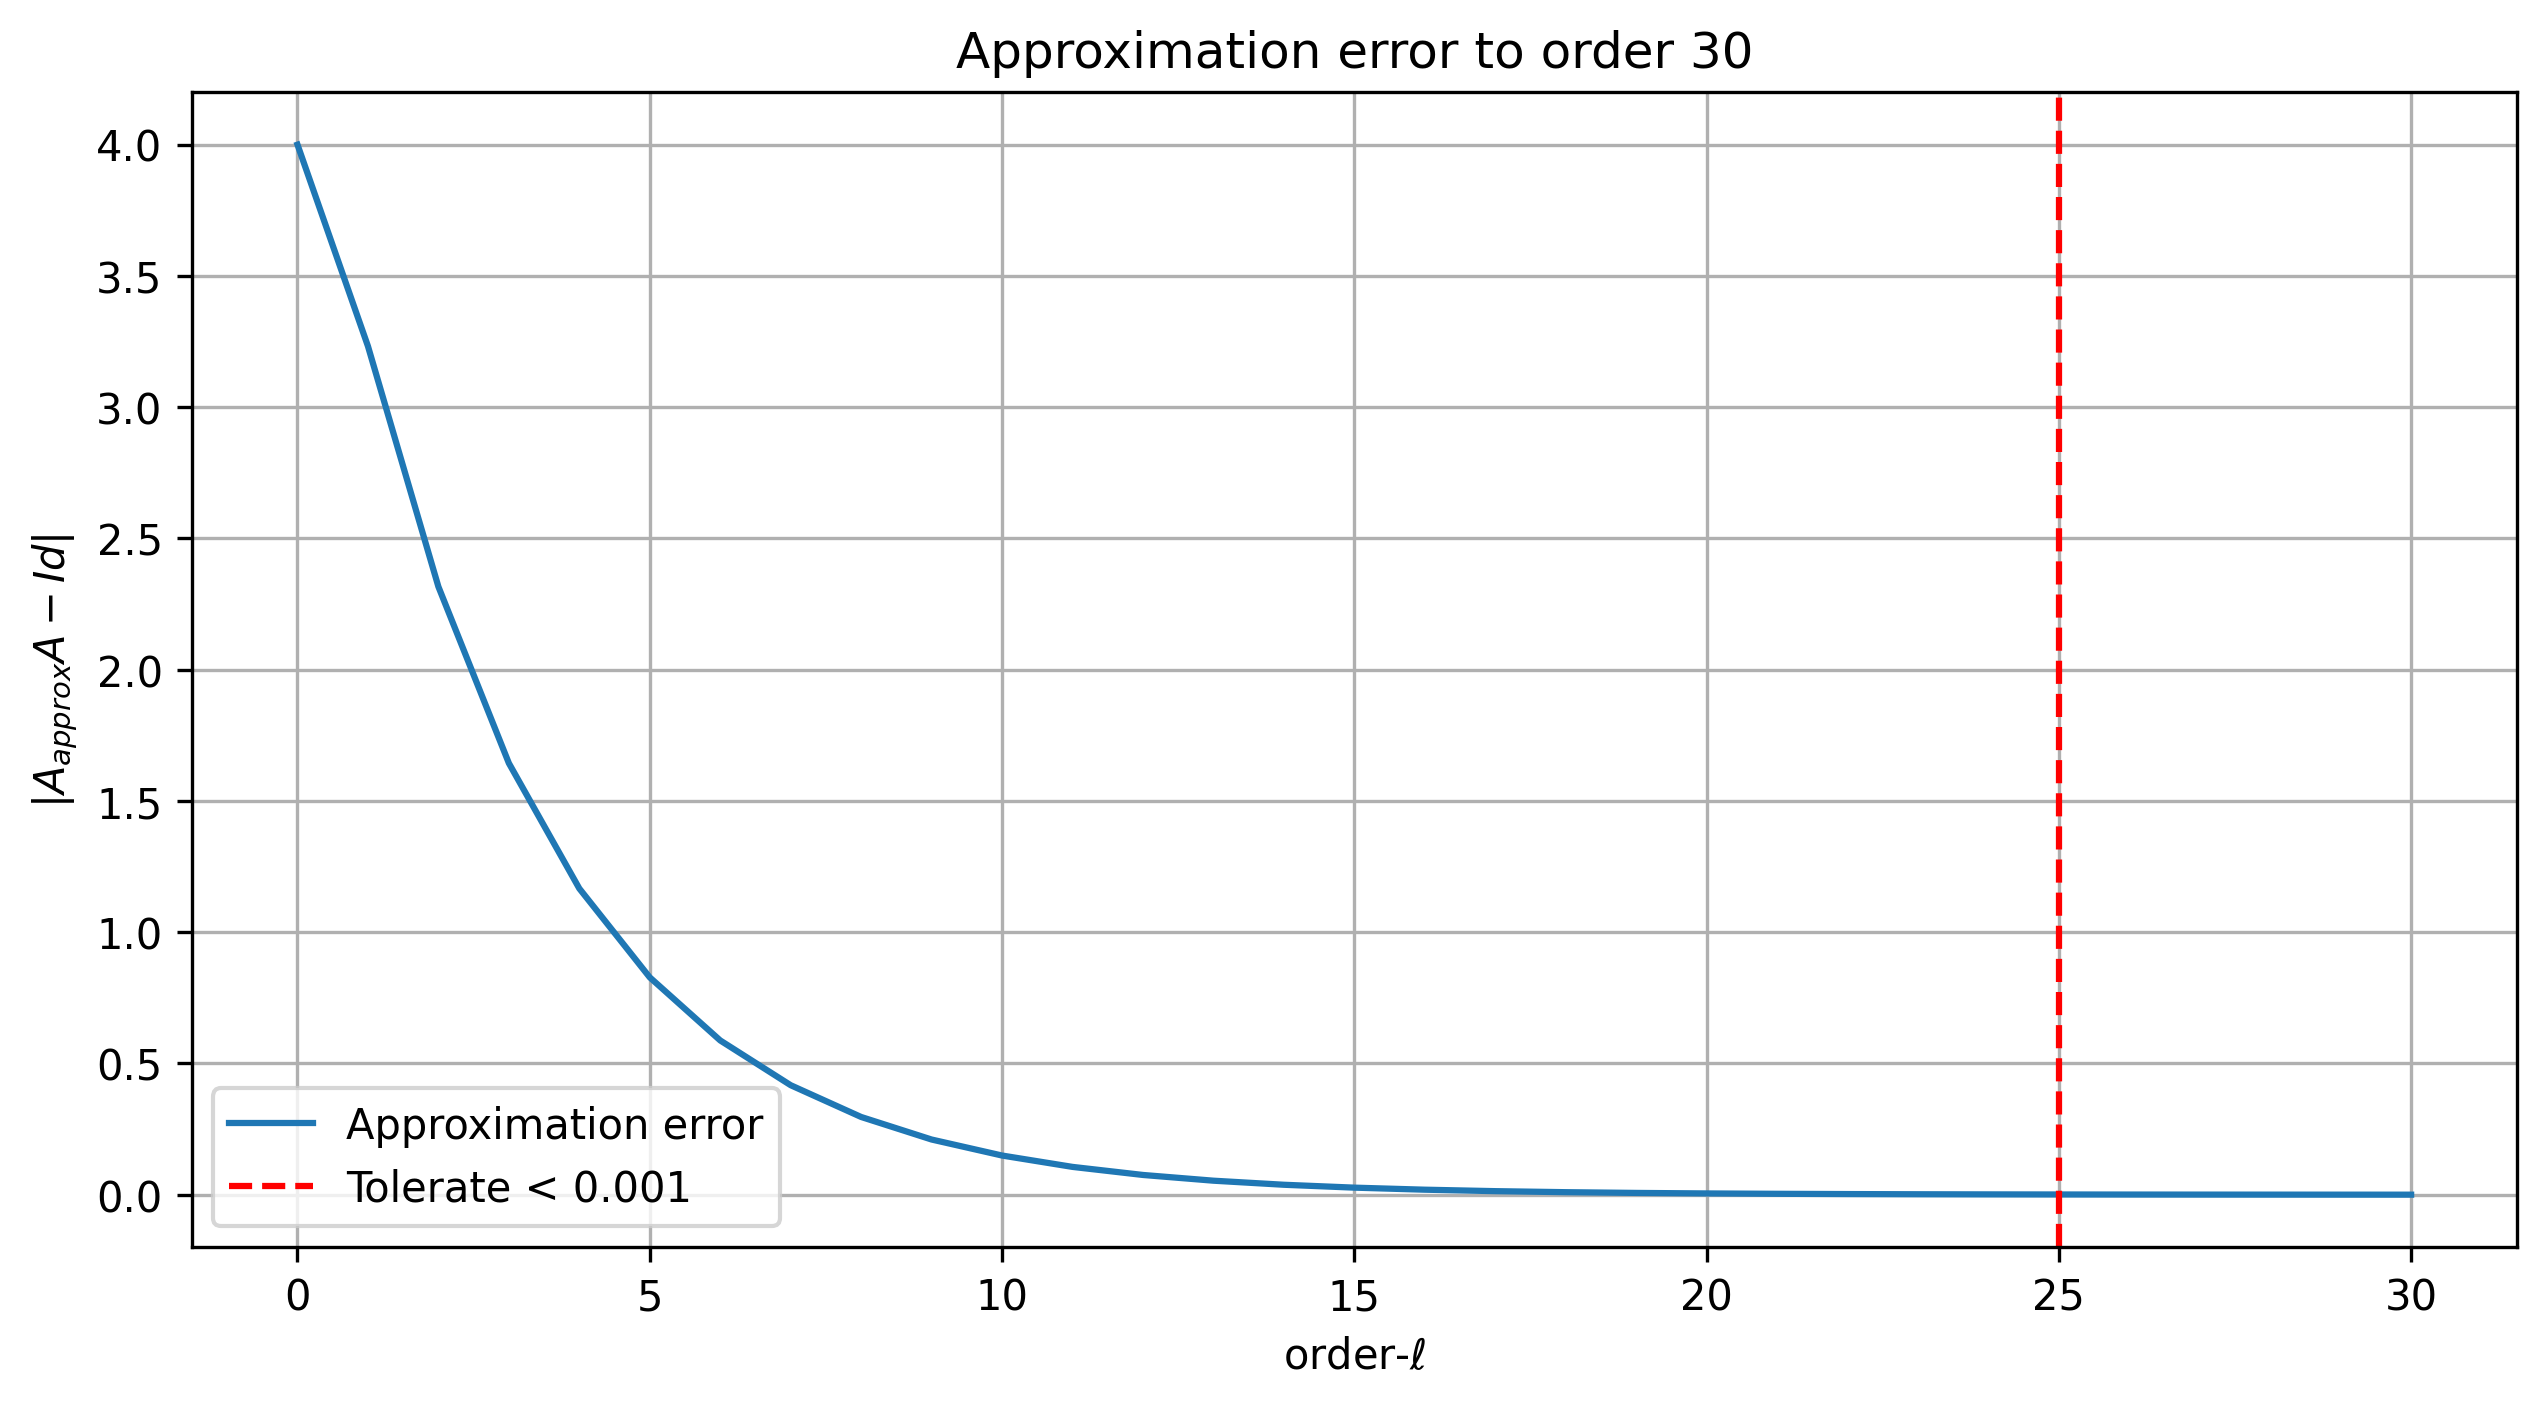
\includegraphics[width=.9\textwidth]{img/results/approx_neumann.png}
    \caption{
        Sai số của xấp xỉ ma trận tới bậc $30$.
    }
\end{figure}

Sử dụng $seed = 0$ như trong cài đặt của bài báo, ta có được một xấp xỉ nghịch đảo của ma trận tại bậc $25$ khá tốt khi mức sai số cho phép (tolerate) bé hơn $0.001$, mặc dù từ bậc $15$ thì sai số của xấp xỉ giảm không đáng kể. Sai số của xấp xỉ được tính bằng tổng sai khác của tích ma trận gốc và ma trận được xấp xỉ với lại ma trận đơn vị.
% np.sum(np.abs(np.dot(matrix, matrix_approx) - I))
    
Với các trường hợp bán kính phổ của ma trận lớn hơn $1$, chuỗi Neumann không hội tụ, nên không thể xấp xỉ ma trận được. Trong bài báo, dữ liệu được tạo ra với một ma trận hiệp phương sai với bán kính phổ lớn hơn $1$. Sở dĩ bài báo không quan tâm tới bán kính phổ lớn hơn $1$ 
là vì mạng NeuMiss sử dụng các ma trận trọng số để học và xấp xỉ sao cho các lớp ma trận trọng số sẽ tương ứng với xấp xỉ nghịch đảo $\cov_{obs}^{-1}$, không bắt buộc bán kính phổ ma trận hiệp phương sai nhỏ hơn $1$ để hoạt động. Nên trong code tạo dữ liệu của tác giả, không có điều kiện kiểm tra bán kính phổ nhỏ hơn $1$.


\subsection{Mạng NeuMiss}
Ta tiến hành kiểm tra độ hiệu quả của mạng NeuMiss trên tập dữ liệu 
được sinh ra từ phân phối chuẩn đa biến, với $Y$ được tính bằng hàm tuyến tính của $X$ như trong phương trình \eqref{eq:lr_matrix_notation}, cùng với $50\%$ dữ liệu bị khuyết ngẫu nhiên (MCAR) ở mỗi đặc trưng trong tập dữ liệu và nhiễu $\varepsilon$ tuân theo phân phối chuẩn với tỷ lệ signal-to-noise (SNR) bằng~$10$ (tỷ lệ nhiễu nhỏ hơn $10$ lần so với ``tín hiệu'' $Y$).

Do dữ liệu được sinh ra từ mô hình tuyến tính, nên bài báo sử dụng metric $R$ bình phương (R-squared -- $R^2$), hay còn được gọi là hệ số xác định (coefficient of determination), để tính 
tỷ lệ của độ biến thiên cho biến phụ thuộc $Y$ được giải thích bởi biến độc lập $X$, từ đó đánh giá độ hiệu quả của mô hình. 

Ngoài ra, ta còn có các biến thể khác của $R^2$ như:
\begin{itemize}
    \item $R^2$ hiệu chỉnh (Adjusted R-squared) cho ta biết được tỷ lệ biến thiên được giải thích chỉ bằng các biến độc lập thật sự ảnh hưởng tới biến phụ thuộc.
    \item $R^2$ cho dự đoán (Predicted R-Squared) cho biết độ chính xác của mô hình trên tập dữ liệu chưa biết.
\end{itemize}

Tuy nhiên, ta không quan tâm tới các mối quan hệ của các biến độc lập với biến phụ thuộc mà chỉ quan tâm tới độ tốt của mô hình trên tập dữ liệu đang xét, nên $R^2$ hiệu chỉnh hay $R^2$ cho dự đoán không được sử dụng trong trường hợp này.

Bayes rate (Tỷ lệ Bayes) là giá trị $R^2$ tốt nhất mà mô hình đạt được dựa trên lý thuyết, được ước lượng thông qua phương trình dự đoán Bayes \eqref{eq:lr_matrix_notation}.
Khi hệ số xác định càng gần với Bayes rate, tức kết quả $R^2 - \text{Bayes rate}$ càng tiến về $0$ thì độ hiệu quả của mô hình càng tốt. 


Sử dụng PyTorch để cài đặt mạng NeuMiss với độ sâu $10$, hàm mất mát là MSE, train (huấn luyện) trên CPU, thời gian train tầm $2$ phút cho 500~epochs, với batch size là~$256$, learning rate là 0.001.
Mạng cho ra chỉ số $R^2$ cho tập train quanh ngưỡng $0.8$, tập validation và test quanh ngưỡng $0.75$.

% Ngoài ra, tác giả chính của bài báo cũng cho ra thêm một bài báo nữa vào năm 2021 \cite{le2021goodimputation}, nói về việc có thể áp dụng NeuMiss cho các mô hình phi tuyến bằng cách huấn luyện nó chung với mô hình MLP sau mạng NeuMiss.


\begin{table}[h!]
\centering
\setlength{\tabcolsep}{10pt}
\begin{tabular}{lcccccc}
\toprule
& \multicolumn{2}{c}{\textbf{Train Set}} & \multicolumn{2}{c}{\textbf{Validation Set}} & \multicolumn{2}{c}{\textbf{Test Set}} \\
\cmidrule(lr){2-3}\cmidrule(lr){4-5}\cmidrule(lr){6-7}
 & $R^2$ & MSE & $R^2$ & MSE & $R^2$ & MSE \\
\midrule
NeuMiss depth-10 & 0.8072 & 0.208 & 0.7482 & 0.2808 & 0.7578 & 0.2674 \\
\bottomrule
\end{tabular}
\captionsetup{justification=centering, width=\linewidth}
\caption{Hiệu suất của NeuMiss với độ sâu 10.}
\label{tab:performance}
\end{table}
% Trong khi đó, Bayes rate cho tập train là $0.8205$ và tập test là $0.8078$. Ta thấy mạng NeuMiss cho ra kết quả khá tốt so với kết quả đạt được của mô hình 


\subsection{Một số kết quả khác}
Sau đây là một số kết quả thực nghiệm khác cho mạng NeuMiss, được train với 500 epochs.

\subsubsection*{So sánh mạng khi có residual connection với khi không có residual connection}\label{section:residual_connection}
Với mạng NeuMiss độ sâu 10:
\begin{table}[h!]
\centering
\setlength{\tabcolsep}{7.3pt}
\begin{tabular}{p{5.3cm}cccccc}
\toprule
& \multicolumn{2}{c}{\textbf{Train Set}} & \multicolumn{2}{c}{\textbf{Validation Set}} & \multicolumn{2}{c}{\textbf{Test Set}} \\
\cmidrule(lr){2-3}\cmidrule(lr){4-5}\cmidrule(lr){6-7}
 & $R^2$ & MSE & $R^2$ & MSE & $R^2$ & MSE \\
\midrule
\raggedright Có residual connection & 0.8116 & 0.2033 & 0.7424 & 0.2873 & 0.7511 & 0.2747 \\
\raggedright Không có residual connection & 0.8257 & 0.1880 & 0.7708 & 0.2556 & 0.7641 & 0.2604 \\
\bottomrule
\end{tabular}
\captionsetup{justification=centering, width=\linewidth}
\caption{Hiệu suất của NeuMiss với độ sâu 10 khi có và không có residual connection.}
\label{tab:performance_residual}
\end{table}

Khi không có residual connection, các chỉ số tốt hơn 1 chút so với khi có residual connection. Có thể do khi mạng có độ sâu lớn, việc có residual connection giúp mạng hoạt động hiệu quả hơn.

Qua đây, ta có thể thấy việc có residual connection không ảnh hướng nhiều tới kết quả so với mạng không có residual connection, như trong bài báo \cite{le2020neumiss} đã đề cập.


\subsubsection*{So sánh các mạng với độ sâu khác nhau}

\begin{table}[h!]
\centering
\setlength{\tabcolsep}{8pt}
\begin{tabular}{ccccccc}
\toprule
\textbf{Độ sâu} & \multicolumn{2}{c}{\textbf{Train Set}} & \multicolumn{2}{c}{\textbf{Validation Set}} & \multicolumn{2}{c}{\textbf{Test Set}} \\
\cmidrule(lr){2-3}\cmidrule(lr){4-5}\cmidrule(lr){6-7}
 & $R^2$ & MSE & $R^2$ & MSE & $R^2$ & MSE \\
\midrule
1  & 0.7823 & 0.2349 & 0.7500 & 0.2788 & 0.7678 & 0.2563 \\
5  & 0.7959 & 0.2202 & 0.7492 & 0.2796 & 0.7586 & 0.2664 \\
10 & 0.8191 & 0.1951 & 0.7548 & 0.2735 & 0.7676 & 0.2565 \\
15 & 0.8164 & 0.1980 & 0.7624 & 0.2650 & 0.7636 & 0.2610 \\
20 & 0.8157 & 0.1988 & 0.7286 & 0.3027 & 0.7431 & 0.2836 \\
\bottomrule
\end{tabular}
\captionsetup{justification=centering, width=\linewidth}
\caption{Hiệu suất của NeuMiss với các độ sâu khác nhau.}
\label{tab:performance-depths}
\end{table}

Mạng NeuMiss càng sâu thì hiện tượng hiệu suất giảm dần (diminishing returns) xuất hiện như trong bài báo \cite{le2020neumiss} đã đề cập. 
Điều này cho thấy việc tăng độ sâu của mạng không đảm bảo sẽ cải thiện kết quả trên tập test.


\subsubsection*{So sánh các mạng với tỷ lệ dữ liệu khuyết khác nhau}
\begin{table}[h!]
\centering
\setlength{\tabcolsep}{8pt}
\begin{tabular}{ccccccc}
\toprule
\textbf{Tỷ lệ khuyết} & \multicolumn{2}{c}{\textbf{Train Set}} & \multicolumn{2}{c}{\textbf{Validation Set}} & \multicolumn{2}{c}{\textbf{Test Set}} \\
\cmidrule(lr){2-3}\cmidrule(lr){4-5}\cmidrule(lr){6-7}
  & $R^2$ & MSE & $R^2$ & MSE & $R^2$ & MSE \\
\midrule
0.1\% & 0.8133 & 0.2014 & 0.7565 & 0.2716 & 0.7506 & 0.2752 \\
0.2\% & 0.8145 & 0.2001 & 0.7533 & 0.2751 & 0.7517 & 0.2741 \\
0.5\% & 0.8191 & 0.1952 & 0.7700 & 0.2565 & 0.7682 & 0.2558 \\
0.8\% & 0.7973 & 0.2187 & 0.7505 & 0.2782 & 0.7572 & 0.2680 \\
\bottomrule
\end{tabular}
\captionsetup{justification=centering, width=\linewidth}
\caption{Hiệu suất của NeuMiss độ sâu 10 với các tỷ lệ khuyết khác nhau.}
\label{tab:performance_missing_rates}
\end{table}

Ta nhận thấy rằng dù tỷ lệ khuyết nhiều nhưng NeuMiss vẫn cho ra kết quả tốt.


\subsubsection*{So sánh các mạng với số lượng mẫu và đặc trưng khác nhau}

\begin{table}[h!]
\centering
\setlength{\tabcolsep}{6pt}
\begin{tabular}{cccccccc}
\toprule
\textbf{Mẫu} & \textbf{Đặc trưng} & \multicolumn{2}{c}{\textbf{Train Set}} & \multicolumn{2}{c}{\textbf{Validation Set}} & \multicolumn{2}{c}{\textbf{Test Set}} \\
\cmidrule(lr){3-4}\cmidrule(lr){5-6}\cmidrule(lr){7-8}
 & & $R^2$ & MSE & $R^2$ & MSE & $R^2$ & MSE \\
\midrule
\multirow{2}{*}{100} & 10 & 0.8609 & 0.1581 & -1.6307 & 2.0416 & -12.7133 & 7.1884 \\
                     & 20 & 0.9450 & 0.0596 & -324.8323 & 205.5099 & -418.3801 & 224.8063 \\
\midrule
\multirow{2}{*}{1000} & 10 & 0.5976 & 0.4539 & -1.5842 & 2.8056 & -0.4908 & 1.6403 \\
                      & 20 & 0.7279 & 0.2953 & -42.1458 & 41.3359 & -64.2313 & 43.3147 \\
\midrule
\multirow{2}{*}{5000} & 10 & 0.8186 & 0.2037 & 0.7657 & 0.2481 & 0.7715 & 0.2491 \\
                      & 20 & 0.8929 & 0.1189 & -0.2029 & 1.3849 & -0.1616 & 1.3378 \\
\midrule
\multirow{2}{*}{10000} & 10 & 0.8138 & 0.2008 & 0.7489 & 0.2800 & 0.7568 & 0.2684 \\
                       & 20 & 0.8783 & 0.1336 & 0.1887 & 0.9035 & 0.2765 & 0.8806 \\
\midrule
\multirow{2}{*}{50000} & 10 & 0.8249 & 0.1933 & 0.8124 & 0.2071 & 0.8001 & 0.2232 \\
                       & 20 & 0.8056 & 0.2153 & 0.7145 & 0.3151 & 0.7282 & 0.3021 \\
\bottomrule
\end{tabular}
\captionsetup{justification=centering, width=\linewidth}
\caption{Hiệu suất của NeuMiss độ sâu 10 với các tuỳ chỉnh số lượng mẫu và đặc trưng khác nhau cho tập dữ liệu.}
\label{tab:performance_grouped_samples_features}
\end{table}

Qua Bảng \ref{tab:performance_grouped_samples_features}, ta thấy rằng mạng NeuMiss chỉ hoạt động tốt khi số lượng mẫu ở mức trung bình trở lên. Điều này cho thấy mạng NeuMiss phù hợp với các tập dữ liệu trung bình, như trong bài báo \cite{le2020neumiss} đã đề cập.


\subsubsection*{So sánh với các phương pháp khác}
Ta so sánh mạng NeuMiss với các phương pháp điền khuyết kết hợp việc sử dụng mô hình hồi quy tuyến tính để dự đoán. 
Các phương pháp này được cài đặt thông qua thư viện \textit{fancyimpute}\footnote{\href{https://pypi.org/project/fancyimpute/}{https://pypi.org/project/fancyimpute/}}, \textit{scikit-learn}\footnote{\href{https://pypi.org/project/scikit-learn/}{https://pypi.org/project/scikit-learn/}}, với kết quả tốt nhất được chọn từ nhiều tuỳ chỉnh khác nhau.
Các kết quả được so sánh với hiệu suất của mạng NeuMiss ở bảng \ref{tab:performance}, sử dụng chỉ số $R^2$ để đánh giá trên tập train và tập test. 

\begin{table}[h!]
\centering
\setlength{\tabcolsep}{10pt}
\begin{tabular}{lcc}
\toprule
& \multicolumn{1}{c}{\textbf{Train Set}} 
& \multicolumn{1}{c}{\textbf{Test Set}} \\
% \cmidrule(lr){2-3}\cmidrule(lr){4-5}\cmidrule(lr){6-7}
 % & $R^2$ & MSE & $R^2$ & MSE \\
\midrule
NeuMiss depth-10 & \textbf{0.8072}  & \textbf{0.7578} \\
KNN imputer + LR & 0.6929 & 0.7018 \\
Simple imputer + LR & 0.6574 & 0.6478 \\
SoftImpute + LR & 0.7604 & 0.7524 \\
MissForest + LR & 0.7708 & 0.7442 \\
MICE + LR & 0.7496 & 0.7313 \\
Simple imputer + MLP regressor & 0.8022 & 0.7330 \\

\bottomrule
\end{tabular}
\captionsetup{justification=centering, width=\linewidth}
\caption{Hiệu suất của NeuMiss độ sâu 10 với các phương pháp khác.}
\label{tab:performance-others}
\end{table}

Qua các kết quả này, ta có thể thấy mạng NeuMiss tỏ ra vượt trội hơn so với các phương pháp điền khuyết truyền thống.
